\documentclass[a4paper,11pt,twoside]{book}

\usepackage[english]{babel}
\usepackage{setspace}
\usepackage[utf8]{inputenc}
\usepackage{graphicx}
\usepackage{pdfpages}
\usepackage{longtable}
\usepackage{url}
\urlstyle{tt}

\usepackage{hyperref}
\usepackage{fullpage}
\usepackage{fancyhdr}

\hypersetup{
     colorlinks = true, linkcolor = blue,
     citecolor   = blue,
     urlcolor    = blue,
}


\usepackage{tocloft}
\renewcommand{\cftpartleader}{\cftdotfill{\cftdotsep}} % for parts
\renewcommand{\cftchapleader}{\cftdotfill{\cftdotsep}} % for chapters
\renewcommand{\cftsecleader}{\cftdotfill{\cftdotsep}} % for sections

\renewcommand{\headrulewidth}{0pt}

\newcommand{\newoddpage} {\clearpage
  \ifthenelse{\isodd{\value{page}}}{}
  {\thispagestyle{empty}\quad\newpage}}

\newcommand{\addpaper}[5]{% #1 path; #2 label; #3 authors; #4 title; #5 URL
  \newoddpage
  \phantomsection
  \addcontentsline{toc}{section}{#3. \emph{#4}}  

\thispagestyle{fancy} %
  
  % scriptsize / tiny
  \lfoot{\scriptsize {\tiny Martins, Moniz, Fumega, Martins, Batista, Coheur, Parra, Trancoso, Turchi, Bisazza, Moorkens, Guerberof, Nurminen, Marg, Forcada (eds.)}\\
    {\em Proceedings of the 22nd Annual Conference of the European Association for Machine Translation}, p. \pageref{beg#2}--\pageref{end#2}\\
      Lisboa, Portugal, November 2020. %\url{#5}
  }
  \cfoot{}
  %
  \label{beg#2}
  \includepdf[pages={1},pagecommand={},fitpaper=true,trim=0 0 0 0,
  offset=0 0, turn=true,noautoscale=true]{#1}
  %
  \pagestyle{fancy} %
  \lfoot{} %
  \cfoot{\thepage} 
  %
  \includepdf[pages={2-},pagecommand={\label{end#2}},fitpaper=true,trim=0 0
  0 0, offset=0 0,turn=true,noautoscale=true]{#1}
}


\newcommand{\addproject}[5]{% #1 path; #2 label; #3 authors; #4 title;
                          % #5 URL
  \newoddpage
  \phantomsection
  \addcontentsline{toc}{section}{#3. \emph{#4}}  
  \thispagestyle{fancy} %
  \lfoot{\scriptsize {\tiny Martins, Moniz, Fumega, Martins, Batista, Coheur, Parra, Trancoso, Turchi, Bisazza, Moorkens, Guerberof, Nurminen, Marg, Forcada (eds.)}\\
    {\em Proceedings of the 22nd Annual Conference of the European Association for Machine Translation}, p. \pageref{beg#2}\\
      Lisboa, Portugal, November 2020. %\url{#5}
  }
  \cfoot{}
  %
  \label{beg#2}
  \includepdf[pages={1},pagecommand={},fitpaper=true,trim=0 0 0 0,
  offset=0 0, turn=true,noautoscale=true]{#1}
  %
  \pagestyle{fancy} %
  \lfoot{} %
  \cfoot{\thepage} 
}


\usepackage{calc}
\setlength{\footskip}{\paperheight
  -(1in+\voffset+\topmargin+\headheight+\headsep+\textheight)
  -0.6in}

\newcommand{\mychapter}[1]{
    \newpage
    \phantomsection{}
    \cfoot{}
    \vspace*{\fill}
    \begin{center}
    \begin{Huge}
    \textbf{#1}
    \end{Huge}
    \end{center}
    \addcontentsline{toc}{chapter}{#1}
    \vspace*{\fill}
    \newpage
    \cfoot{\thepage}
}

%%%%%%%%%%%%%%%%%%%%%%%%%%%%%%%%%%%%%%%%%%%%%%%%%%%%%%%%%%%%%%%828%%%%%%%%%%%%%%%%%

%\usepackage{draftwatermark}
%\SetWatermarkText{Draft}
%\SetWatermarkScale{1}

\begin{document}

\pagestyle{fancy} 
\lhead{}
\rhead{}
\chead{}
\lfoot{} 
\rfoot{} 
\cfoot{\thepage}

\newoddpage
\thispagestyle{empty}
\enlargethispage{1cm}
\begin{center}
\phantom{x}
\vspace{-2cm}

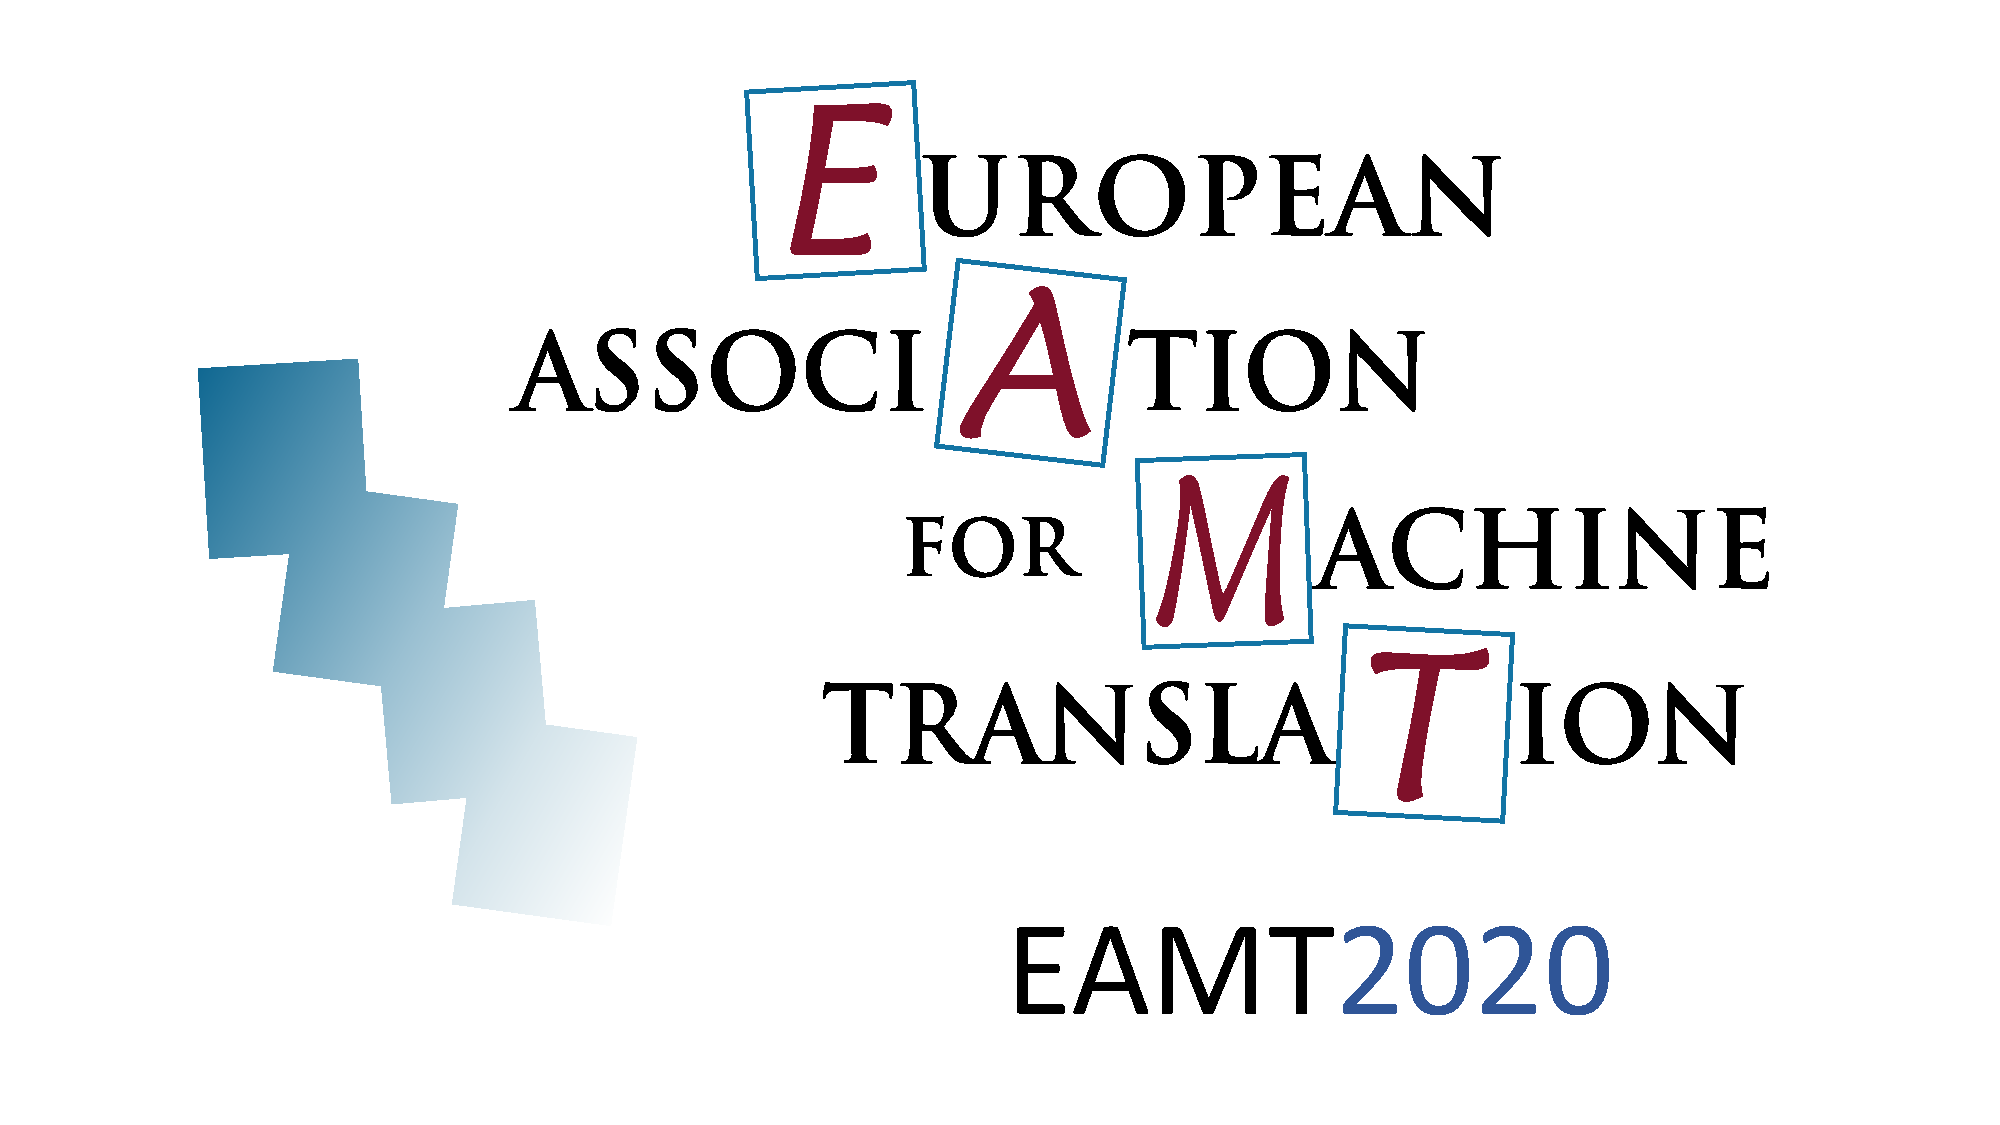
\includegraphics[width=0.8\columnwidth]{logos/eamt2020-lisbon.pdf}

\vspace{1cm}

{\huge Proceedings of the}\\[2ex]
\textbf{\huge 22nd Annual Conference of \\[0.2ex]
  the European Association\\[1.0ex] for Machine Translation} 
  
\vspace{1.5cm}

{\LARGE 3 -- 5 November 2020\\{\bf Online Conference}\\[0.75ex]in place of\\[0.75ex]Instituto Superior Técnico, Lisbon, Portugal}
\vspace{3cm}

\textbf{\em Edited by}

\vspace{1em}
André Martins, 
Helena Moniz,
Sara Fumega,
Bruno Martins,
Fernando Batista,
Luisa Coheur,
Carla Parra,
Isabel Trancoso,
Marco Turchi,
Arianna Bisazza,
Joss Moorkens,
Ana Guerberof,
Mary Nurminen,
Lena Marg,
Mikel L. Forcada

%\vspace{1cm}
\vfill

\textbf{\em Organised by}

\vspace{1em}
\begin{tabular}{ccc}

\includegraphics[width=0.30\columnwidth]{logos/unbabel-logo.png} & 
\includegraphics[width=0.30\columnwidth]{logos/inescid-logo.png} & 
\includegraphics[width=0.30\columnwidth]{logos/ist-logo.png}\\
\end{tabular}
\end{center}

\newoddpage
\thispagestyle{empty}
\vfill \mbox{} \vfill

\begin{onehalfspacing}

\noindent 
\includegraphics[scale=0.5]{logos/creative_commons.pdf} 
\vspace{1em}

\noindent 
The papers published in this proceedings are ---unless indicated
otherwise--- covered by the Creative Commons
Attribution-NonCommercial-NoDerivatives 3.0 International (CC-BY-ND
3.0). You may copy, distribute, and transmit the work, provided that
you attribute it (authorship, proceedings, publisher) in the manner
specified by the author(s) or licensor(s), and that you do not use it
for commercial purposes. The full text of the licence may be found at
\url{https://creativecommons.org/licenses/by-nc-nd/3.0/deed.en}.

\vspace{1cm}

\noindent © 2020 The authors\\
\noindent \textbf{ISBN:} 978-989-33-0589-8\\

\end{onehalfspacing}

\vfill \mbox{}

%%%%%%%%%%%%%%%%%%%%%%%%%%%%%%%%%%%%%%%%%%%%%%%%%%%%%%%%%%%%%%%%%%%%%%%%%%%%%%%%

\newoddpage
\frontmatter

\tableofcontents

\begin{onehalfspacing}

\chapter*{Foreword from the General Chair}
\addcontentsline{toc}{chapter}{Foreword from the General Chair}
%\vspace{-0.8cm}


\noindent
\emph{Bem-vindas e bem-vindos!}\\

As president of the European Association for Machine Translation (EAMT) and General Chair of the 22nd Annual Conference of the EAMT, it's a pleasure for me to write these opening words to the Proceedings of EAMT~2020.

But on the other hand, I have some mixed feeling when I write these lines. Due to the COVID-19 crisis, we have not been able to meet in Lisbon, in person, in May. And that's so sad.

The organizers have reacted swiftly to make EAMT~2020 possible. First, we postponed it in hopes that we would be able to meet in November. But then reality struck and it was clear that not even that would be possible. Finally, it was decided that EAMT~2020 will be an on-line conference, from November 3 to November 5, 2020. We'll still have a single-room conference  (including boaster sessions for papers accepted as posters), and we will do our best to make it as interactive and lively as possible. Details will be published in the EAMT~2020 website. Of course, registration fees have been reduced accordingly.

Reviewing had finished and acceptance decisions had been made, so it didn't make much sense to hold the publication of these Proceedings; here they are! Authors can now freely disseminate the papers in this volume. You can see them as a snapshot of active research and development by the best groups in Europe and around the world --- I am sure authors will add new and interesting results when we \emph{meet}.

You'll soon see an attractive three-day, four-track programme put together by our programme chairs: Arianna Bisazza and Marco Turchi, research track co-chairs, Mary Nurminen and Lena Marg, user track co-chairs, and Ana Guerberof and Joss Moorkens, translator track co-chairs; I thank them for the hard work. Finally, as General Chair, I took care of the fourth track, the projects/products track. The technical coordination of the reviewing was done by Carolina Scarton (thanks, Carol!).  I also feel honored to have Lucia Specia (Imperial College London) as our invited speaker.

To give you a historical note, the EAMT started organizing annual workshops in 1996; later, these workshops became annual conferences, and were hosted all around Europe. Years ago, the venue steadily moved from west to east: from Barcelona (2009) to Saint-Rapha\"{e}l (2010) to Leuven (2011) to Trento (2012) to Dubrovnik (2014) ---after skipping one year to host the successful world-wide MT Summit 2013 in Nice---; then it turned  around to go west again at Antalya (2015),
to go to Riga (2016), then Prague (2017), then Alacant (2018) and now ---after skipping another year to host another successful MT Summit in Dublin--- well, virtually, Lisbon. It's hard to go further westwards, so the next venue will take place east from Lisbon, as we will announce in November.

By the way, if you have not done so yet, and live in Europe, North Africa, or the Middle East,
please consider joining the EAMT. Our membership rates are low, particularly for students
and people not based in Europe. You will benefit from discounts when attending not only
our conferences, but also the conferences held by our partner associations the Asia-Pacific
Association for Machine Translation (AAMT) and the Association for Machine Translation in
the Americas (AMTA). You will also have an exclusive chance to benefit from funding for your
activities related to machine translation. And perhaps you can get even more involved and
participate in serving the European machine translation community by becoming a member of
the Executive Committee of the EAMT.


EAMT 2020 would have never been possible without the generous offer to host and the
hard work subsequently done by the local organizing committee at Unbabel, but also at the \emph{Instituto Superior Técnico}, the \emph{Instituto de Engenharia de Sistemas e Computadores, Investigação e Desenvolvimento} and the \emph{Instituto Universitário de Lisboa}, particularly André Martins, Helena Moniz, Sara Fumega, Bruno Martins, Fernando Batista, Luisa Coheur, Carla Parra Escartín, and Isabel Trancoso.

It is also with great pleasure that I thank our sponsors Banco Português de Investimento (gold sponsor), STAR Group and Microsoft (silver sponsors), Unbabel, text\&form, TAUS, Pangeanic, and Crosslang (bronze sponsors), and Apertium and Prompsit (supporting sponsors), particularly for the flexibility shown when adapting to the changes in how the conference is run. EAMT 2020 would not be possible without the amazing engagement of these companies. I am also thankful for the ample support received from the local institutions in Lisbon. 

Finally, I would like to thank future EAMT 2020 attendees for participating but also for their understanding. I hope
the conference leads to new friendships ---first virtual, and soon, I hope, face to face--- and all sorts of fruitful collaboration in the field of translation technologies. 

Oh, and please be sure to visit Lisbon when they let us travel freely. It was there waiting for us, and it will be when this nightmare is over. I'm looking forward to it.

\vspace{1cm}

\noindent (I wish we were in) Lisboa, 2020

\vspace{1cm}

\noindent \textbf{Mikel L. Forcada}

\noindent President of the EAMT

\noindent General Chair of EAMT 2020

\noindent Professor of Computer Languages and Systems
\noindent Universitat d'Alacant

\noindent Alacant, Valencian Country, Spain.

\noindent Email: \url{mlf@ua.es}


\chapter*{Message from the Organising Committee Chairs}
\addcontentsline{toc}{chapter}{Message from the Organising Committee Chairs}
%\vspace{-0.9cm}

On behalf of the organising committee, we want to take this opportunity to give you a big thank you for joining us in the 22nd Annual Conference of the European Association for Machine Translation, EAMT 2020. 

Sadly, this year, the COVID-19 crisis forced us to a last minute change, and we won’t be able to welcome you to Lisbon, as we wished so much. However, Unbabel and INESC-ID are extremely proud and honored to host the EAMT conference in fully virtual mode for the first time, from the 3rd to the 5th of November of 2020. 

This was of course a very hard decision. In the hope that we could still host a presencial conference, we started by postponing the dates to the first week of November and securing a venue at Instituto Superior Técnico. However, it later became clear that a physical meeting would be impossible under the current circumstances, and together with the board of the European Association for Machine Translation we decided to make EAMT~2020 an on-line conference, with reduced registration fees. We would like to thank all the support from the European Association for Machine Translation in this process, in particular from its president Mikel Forcada and its secretary Carol Scarton for all their help in making this change happen smoothly. We also thank the sponsors and supporting organizations for their flexibility in adapting to a virtual conference.

We are sure EAMT~2020 will be a success with the contribution of everyone! According to our predictions, we expect this edition of the EAMT conference to have one of the highest number of attendees ever. We will have a single-room conference with live talks and booster sessions for papers accepted as posters. We will do our best to make it as interactive and lively as possible. We will plan for virtual social events keeping the best spirit of Lisbon. Stay tuned!

We look forward to your active participation during the three days of the conference. Do not hesitate to ask questions when the session chairs invite you to do so. Please, contribute to make this edition of the conference a fruitful forum where a multidisciplinary group of researchers, developers, practitioners, leaders, vendors, users, and translators all share experiences and motivating ideas.

Finally, we would like to express our sincere appreciation to the people and organisations that have made this conference possible: the European Association for Machine Translation, in particular Mikel Forcada and Carol Scarton for all their support in changing the conference to virtual mode, our gold sponsor (Banco Português de Investimento), Silver sponsors (STAR Group and Microsoft), Bronze sponsors (Unbabel, Text\&Form, TAUS, Pangeanic, and Crosslang), supporters (Apertium and Prompsit), institutional partners Unbabel, \emph{Instituto Superior Técnico}, the \emph{Instituto de Engenharia de Sistemas e Computadores, Investigação e Desenvolvimento} and the \emph{Instituto Universitário de Lisboa}, programme chairs (Marco Turchi, Arianna Bisazza, Joss Moorkens, Ana Guerberof, Mary Nurminen, and Lena Marg), keynote speaker (Lucia Specia), and, finally but so importantly, our colleagues Sara Fumega, Bruno Martins, Fernando Batista, Luisa Coheur, Carla Parra Escartín, and Isabel Trancoso, who have worked extraordinarily hard to make this conference as pleasant and inspiring as possible. 


%\vspace{1cm}
%\begin{center}
%\begin{tabular}{p{5cm}p{5cm}}
%André Martins & Helena Moniz\\
%IST and Unbabel & INESC-ID and Unbabel\\
%\end{tabular}
%\end{center}


\vspace{1cm}
\begin{center}
\setlength{\tabcolsep}{20pt}
\begin{tabular}{ll}
André Martins		&  Helena Moniz\\
IST and Unbabel	& INESC-ID and Unbabel\\
\end{tabular}
\end{center}


\chapter*{Preface by the Programme Chairs}
\addcontentsline{toc}{chapter}{Preface by the Programme Chairs}

It is our pleasure to welcome you to the 22nd annual conference of the European Association for Machine Translation (EAMT) to be held remotely from November 3 to 5, 2020. Organizing this edition in the time of a pandemic that brought about traveling and many other restrictions has been a sort of roller coaster. The whole organizing committee has worked hard to maintain the usual standards of quality and confirm the EAMT conference as the most important event in Europe in the area of machine translation for researchers, users and professional translators.

Following the success of the previous edition, this year once again there are four tracks: research, user, translators, and project/product. The research track concerns novel and significant research results in any aspect of MT and related areas while the user track reports users’ experiences with MT in industry, government, NGOs, as well as innovative uses of MT. The translator track focuses on translators’ interaction with MT, including MT evaluation using professional translators, post-editing practices and tools, usability, and pricing. The project/product track offers projects and products the opportunity to be presented to the wide audience of the conference.

This year we have received 47 submissions to the research track, 15 submissions to the user track, 13 submissions to the translators’ track, and 22 descriptions of projects and products. Each submission to the research, user and translator tracks was peer reviewed by two or three independent members of the Programme Committee depending on the specific track. In the research track, 25 papers (53\%) were accepted for publication, whereas 12 papers (80\%) were accepted for the user track, and 9 papers (69\%) for the translators track. 
Aside from regular papers from the four tracks, the programme includes an invited talk by Lucia Specia, from the University of Sheffield and Imperial College London, on “Exploring NMT’s bag of tricks for translation quality estimation and evaluation”. We will also have a presentation by the winner of the EAMT Best Thesis Award, Felix Stahlberg, with his thesis "The Roles of Language Models and Hierarchical Models in Neural Sequence-to-Sequence Prediction" (University of Cambridge).

We would like to thank everyone who, by offering their flexibility and extra efforts, made it possible to deal with continuously moving deadlines. In particular, we thank the Programme Committee members whose names are listed below for their high-quality reviews and recommendation which have been very useful for the Programme Chairs to make decisions. We would also like to thank all the authors for trying their best to incorporate the reviewers’ suggestions when preparing the final versions of their papers. For the papers which were not accepted, we hope that the reviewers’ comments will be useful for improving them. Finally, thanks to Mikel Forcada and Carol Scarton for all of their help and advice!

\vspace{1cm}
\begin{center}
\setlength{\tabcolsep}{20pt}
\begin{tabular}{ll}
Arianna Bisazza 		& Ana Guerberof-Arenas\\
University of Groningen	& University of Surrey \\
\\
\\
Joss Moorkens			& Marco Turchi\\
Dublin City University	& Fondazione Bruno Kessler\\
\end{tabular}

\end{center}

\end{onehalfspacing}


\chapter*{EAMT 2020 Committees}
\addcontentsline{toc}{chapter}{EAMT 2020 Committees}

\section*{General Chair}
\noindent Mikel L. Forcada, Universitat d’Alacant


\section*{Programme Chairs}
\subsection*{Research track}
\noindent Marco Turchi, FBK\\
\noindent Arianna Bisazza, Groningen Univ.

\subsection*{User track}
\noindent Mary Nurminen, Tampere University\\
\noindent Lena Marg, Welocalize

\subsection*{Translators' track}
\noindent Joss Moorkens, DCU\\
\noindent Ana Guerberof, Univ. of Surrey

\section*{Organising committee}
\noindent André Martins, IST and Unbabel (co-chair)\\
\noindent Helena Moniz, INESC-ID and Unbabel (co-chair)\\
\noindent Sara Fumega, Unbabel\\
\noindent Bruno Martins, IST and INESC-ID\\
\noindent Fernando Batista, INESC-ID and ISCTE-UL\\
\noindent Luisa Coheur, IST and INESC-ID\\
\noindent Isabel Trancoso, IST and INESC-ID

\pagebreak

\section*{Programme Committee}
\subsection*{Research track}

\noindent Tamer Alkhouli, RWTH Aachen University\\
\noindent Mihael Arcan, National University of Ireland Galway\\
\noindent Duygu Ataman, University of Zürich\\
\noindent Anabela Barreiro, INESC-ID\\
\noindent Rachel Bawden, The University of Edinburgh\\
\noindent Núria Bel, Universitat Pompeu Fabra\\
\noindent Luisa Bentivogli, Fondazione Bruno Kessler\\
\noindent José G. C. de Souza, eBay Inc.\\
\noindent Iacer Calixto, University of Amsterdam\\
\noindent Michael Carl, Kent State University\\
\noindent Helena Caseli, Federal University of São Carlos (UFSCar)\\
\noindent Sheila Castilho, Dublin City University\\
\noindent Mauro Cettolo, Fondazione Bruno Kessler\\
\noindent Boxing Chen, Alibaba Group\\
\noindent Colin Cherry, National Research Council Canada\\
\noindent Vishal Chowdhary, Microsoft\\
\noindent Chenhui Chu, Osaka University\\
\noindent Joke Daems, Ghent University\\
\noindent Mattia Antonino Di Gangi, Fondazione Bruno Kessler, University of Trento\\
\noindent Christian Dugast, tech2biz\\
\noindent Cristina España-Bonet, UdS and DFKI\\
\noindent Miquel Esplà, Universitat d'Alacant\\
\noindent Mireia Farrús, Universitat Pompeu Fabra\\
\noindent Marcello Federico, Amazon AI\\
\noindent Orhan Firat, Google\\
\noindent Mark Fishel, University of Tartu\\
\noindent George Foster, Google\\
\noindent Markus Freitag, Google AI\\
\noindent Roman Grundkiewicz, The University of Edinburgh\\
\noindent Nizar Habash, Columbia University\\
\noindent Barry Haddow, The University of Edinburgh\\
\noindent Gholamreza Haffari, Simon Fraser University\\
\noindent Teresa Herrmann, Fujitsu\\
\noindent Vu Hoang, The University of Melbourne\\
\noindent Christopher Hokamp, CNGL - Dublin City University\\
\noindent Matthias Huck, Ludwig Maximilian University of Munich\\
\noindent Julia Ive, King’s College London\\
\noindent Shahram Khadivi, eBay\\
\noindent Philipp Koehn, Johns Hopkins University\\
\noindent Julia Kreutzer, Google AI\\
\noindent Roland Kuhn, National Research Council of Canada\\
\noindent Anoop Kunchukuttan, Microsoft\\
\noindent Surafel Melaku Lakew, University of Trento\\
\noindent Alon Lavie, Carnegie Mellon University\\
\noindent Gregor Leusch, eBay\\
\noindent Samuel Läubli, University of Zurich\\
\noindent Lieve Macken, Ghent University\\
\noindent Andreas Maletti, Universität Leipzig\\
\noindent Daniel Marcu, ISI/USC\\
\noindent Antonio Valerio Miceli Barone, University of Edinburgh\\
\noindent Joss Moorkens, Dublin City University\\
\noindent Mathias Müller, University of Zurich\\
\noindent Maria Nadejde, The University of Edinburgh\\
\noindent Matteo Negri, Fondazione Bruno Kessler\\
\noindent Jan Niehues, Maastricht University\\
\noindent Sharon O'Brien, Dublin City University\\
\noindent Constantin Orasan, University of Surrey\\
\noindent Daniel Ortiz-Martínez, Universitat Politecnica de Valencia\\
\noindent Myle Ott, Facebook\\
\noindent Carla Parra Escartín, Unbabel, Lda.\\
\noindent Pavel Pecina, Charles University In Prague\\
\noindent Stephan Peitz, Apple\\
\noindent Sergio Penkale, Lingo24\\
\noindent Martin Popel, UFAL, Charles University\\
\noindent Andrei Popescu-Belis, HEIG-VD / HES-SO\\
\noindent Maja Popovic, ADAPT Centre @ DCU\\
\noindent Marta R. Costa-Jussà, Institute For Infocomm Research\\
\noindent Matīss Rikters, Tilde\\
\noindent Rudolf Rosa, Charles University\\
\noindent Germán Sanchis-Trilles, Sciling S.L.\\
\noindent Yves Scherrer, University of Helsinki\\
\noindent Rico Sennrich, University of Zurich\\
\noindent Dimitar Shterionov, Dublin City University\\
\noindent Patrick Simianer, Lilt, Inc.\\
\noindent Felix Stahlberg, Google Research\\
\noindent Dario Stojanovski, Ludwig Maximilian University of Munich\\
\noindent Víctor M. Sánchez-Cartagena, Universitat d'Alacant\\
\noindent Felipe Sánchez-Martínez, Universitat d'Alacant\\
\noindent Aleš Tamchyna, Memsource a. s.\\
\noindent Jörg Tiedemann, University of Helsinki\\
\noindent Antonio Toral, University of Groningen\\
\noindent Ke Tran, Amazon\\
\noindent Francis M. Tyers, Indiana University Bloomington\\
\noindent Vincent Vandeghinste, Instituut voor de Nederlandse Taal // Centre for Computational Linguistics, KU Leuven\\
\noindent David Vilar, Amazon\\
\noindent Martin Volk, University of Zurich\\
\noindent Marion Weller-Di Marco, CIS - University of Munich\\
\noindent François Yvon, LIMSI/CNRS et Université Paris-Sud\\
\noindent Jiajun Zhang, Institute of Automation Chinese Academy of Sciences

\pagebreak

\subsection*{User track}
\noindent Nora Aranberri, University of the Basque Country\\
\noindent Adam Bittlingmayer, ModelFront\\
\noindent Bianka Buschbeck, Systran\\
\noindent Dave Clarke, Welocalize\\
\noindent Michael Denkowski, Amazon\\
\noindent Félix Do Carmo, University of Surrey\\
\noindent Thierry Etchegoyhen, Vicomtech-IK4\\
\noindent Valeria Filippello, SDL\\
\noindent Federico Gaspari, Università per Stranieri “Dante Alighieri” di Reggio Calabria\\
\noindent Kim Harris\\
\noindent Georg Kirchner, Dell \\
\noindent Maarit Koponen, University of Helsinki\\
\noindent László Laki, Globalese\\
\noindent Jay Marciano, Lionbridge\\
\noindent Marianna Martindale, University of Maryland\\
\noindent Morgan O’Brien, McAfee\\
\noindent Niko Papula, Multilizer\\
\noindent Daniel Prou, European Commission\\
\noindent Gema Ramírez-Sánchez, Prompsit Language Engineering\\
\noindent Steve Richardson, The Church of Jesus Christ of Latter-day Saints\\
\noindent Jon Ritzdorf, Moravia\\
\noindent Laura Rossi, LexisNexis\\
\noindent Yury Sharshov, LexisNexis Univentio\\
\noindent Dimitar Shterionov, Dublin City University\\
\noindent Charlotte Tesselaar, LexisNexis Univentio\\
\noindent Joachim Vandenbogaert, Crosslang\\
\noindent Andy Way, ADAPT Centre, Dublin City University\\
\noindent Chris Wendt, Microsoft\\
\noindent Masaru Yamada, Kansai University\\
\noindent Anna Zaretskaya, TransPerfect

\subsubsection*{Subreviewers}
\noindent Natasha Latysheva, Welocalize

\clearpage

\subsection*{Translators' track}
\noindent Khetam Alsharou, Imperial College London\\
\noindent Frank Austermuhl, Aston University\\
\noindent Sarah Bawa Mason, University of Portsmouth\\
\noindent Sarah Berthaud, Galway-Mayo Institute of Technology\\
\noindent Pat Cadwell, Dublin City University\\
\noindent Sheila Castilho, Dublin City University\\
\noindent Joke Daems, Ghent University\\
\noindent Christophe Declercq, KU Leuven\\
\noindent Félix do Carmo, University of Surrey\\
\noindent Gökhan Dogru, Universitat Autònoma de Barcelona\\
\noindent Joanna Drugan, University of East Anglia\\
\noindent Maria Fernandez Parra, Swansea University\\
\noindent Joanna Gough, University of Surrey\\
\noindent Dorothy Kenny, Dublin City University\\
\noindent Maarit Koponen, University of Helsinki\\
\noindent Ralph Krüger, TH Köln\\
\noindent Carlos la Orden Tovar, InsideLoc\\
\noindent Claire Larsonneur, Université Paris 8\\
\noindent Krzysztof Loboda, Jagiellonian University\\
\noindent Rudy Loock, Université de Lille\\
\noindent Lieve Macken, Ghent University\\
\noindent Javier Mallo, Freelance Spanish Language Consultant\\
\noindent Giulia Mattoni, Vistatec\\
\noindent Lucas Nunes Vieira, University of Bristol\\
\noindent Sharon O'Brien, Dublin City University\\
\noindent Antoni Oliver, Universitat Oberta de Catalunya\\
\noindent Maeve	Olohan, University of Manchester\\
\noindent Constantin Orasan, University of Surrey\\
\noindent David Orrego Carmona, Aston University\\
\noindent Carla Parra Escartín, Unbabel\\
\noindent Mary Phelan, Dublin City University\\
\noindent Rubén Rodríguez de la Fuente, PayPal\\
\noindent Alessandra Rossetti, Dublin City University\\
\noindent Caroline Rossi, Université Grenoble Alpes\\
\noindent Andrew Rothwell, Swansea University\\
\noindent Akiko Sakamoto, University of Portsmouth\\
\noindent Vilelmini Sosoni, Ionian University\\
\noindent Carlos Teixeira, IOTA Localization Services and Trinity College Dublin


\newoddpage
\mainmatter

\chapter*{Invited Speech}
\addcontentsline{toc}{chapter}{Invited Speech}

\section*{Exploring NMT's bag of tricks for translation quality estimation and evaluation}\label{invited}
Lucia Specia, Imperial College and Sheffield University, UK
\vspace{0.5cm}

\begin{onehalfspacing}

Neural machine translation (NMT) has become the de facto automated translation technology for language pairs where enough parallel data is available. Nevertheless, translation models are not bulletproof. Given the generally very fluent translations produced by these models, automatically assessing their general quality is arguably more challenging, yet paramount. In this talk I will argue that the solution to this problem can to a large extent be provided by NMT models themselves. I will discuss experiments demonstrating that such models provide valuable information for both translation evaluation and quality estimation. Namely, they allow for better supervised as well as fully unsupervised quality estimation models, as well as more for reliable multi-reference evaluation approaches.

\end{onehalfspacing}


\chapter*{EAMT 2019 Best Thesis Award --- Anthony C Clarke Award}
\addcontentsline{toc}{chapter}{EAMT 2019 Best Thesis Award --- Anthony C Clarke Award}

\begin{onehalfspacing}

Ten PhD theses defended in 2019 were received as candidates for the 2019 edition of the Anthony C Clarke Award - EAMT Best Thesis Award, and all ten were eligible. 36 reviewers and six EAMT Executive Committee members were recruited to examine and score the theses, considering how challenging the problem tackled in each thesis was, how relevant the results were for machine translation as a field, and what the strength of its impact in terms of scientific publications was. Two EAMT Executive Committee members also analysed all theses.

The year of 2019 was again a very good year for PhD theses in machine translation. The scores of the best theses were very close, which made it very hard to select a winner. A panel of five EAMT Executive Committee members (André Martins, Lucia Specia, Khalil Sima'an, Carolina Scarton, and Mikel L. Forcada) was assembled to process the reviews and select a winner.

The panel has decided to grant the 2019 edition of the EAMT Best Thesis Award, Anthony C Clarke Award, to {\bf Felix Stahlberg} for his thesis “The Roles of Language Models and Hierarchical Models in Neural Sequence-to-Sequence Prediction”, University of Cambridge, supervised by Bill Byrne.

\end{onehalfspacing}

\addpaper{misc/EAMT_Best_Thesis_Abstract.pdf}{btaw}{Felix Stahlberg}{The Roles of Language Models and Hierarchical Models in Neural Sequence-to-Sequence Prediction}{}

\mychapter{Research papers}

\addpaper{papers_research/EAMT_2020_paper_21.pdf}{pr21}{Alessandra Rossetti, Sharon O'Brien and Patrick Cadwell}{Comprehension and Trust in Crises: Investigating the Impact of Machine Translation and Post-Editing}{}
\addpaper{papers_research/EAMT_2020_paper_29.pdf}{pr29}{Tom Kocmi and Ondřej Bojar}{Efficiently Reusing Old Models Across Languages via Transfer Learning}{}
\addpaper{papers_research/EAMT_2020_paper_34.pdf}{pr34}{Hao Yang, Minghan Wang, Ning Xie, Ying Qin and Yao Deng}{Efficient Transfer Learning for Quality Estimation with Bottleneck Adapter Layer}{}
\addpaper{papers_research/EAMT_2020_paper_36.pdf}{pr36}{Yunsu Kim, Miguel Graça and Hermann Ney}{When and Why is Unsupervised Neural Machine Translation Useless?}{}
\addpaper{papers_research/EAMT_2020_paper_43.pdf}{pr43}{Maciej Modrzejewski, Miriam Exel, Bianka Buschbeck, Thanh-Le Ha and Alexander Waibel}{Incorporating External Annotation to improve Named Entity Translation in NMT}{}
\addpaper{papers_research/EAMT_2020_paper_46.pdf}{pr46}{Minghan Wang, Hao Yang, Ying Qin, Shiliang Sun and Yao Deng}{Unified Humor Detection Based on Sentence-pair Augmentation and Transfer Learning}{}
\addpaper{papers_research/EAMT_2020_paper_49.pdf}{pr49}{Víctor M. Sánchez-Cartagena, Mikel L. Forcada and Felipe Sánchez-Martínez}{A multi-source approach for Breton–French hybrid machine translation}{}
\addpaper{papers_research/EAMT_2020_paper_50.pdf}{pr50}{Allen Antony, Arghya Bhattacharya, Jaipal Goud and Radhika Mamidi}{Leveraging Multilingual Resources for Language Invariant Sentiment Analysis}{}
\addpaper{papers_research/EAMT_2020_paper_66.pdf}{pr66}{Lukas Edman, Antonio Toral and Gertjan van Noord}{Low-Resource Unsupervised NMT: Diagnosing the Problem and Providing a Linguistically Motivated Solution}{}
\addpaper{papers_research/EAMT_2020_paper_70.pdf}{pr70}{Jihyung Moon, Hyunchang Cho and Eunjeong L. Park}{Revisiting Round-trip Translation for Quality Estimation}{}
\addpaper{papers_research/EAMT_2020_paper_72.pdf}{pr72}{Yuting Zhao, Mamoru Komachi, Tomoyuki Kajiwara and Chenhui Chu}{Double Attention-based Multimodal Neural Machine Translation with Semantic Image Regions}{}
\addpaper{papers_research/EAMT_2020_paper_73.pdf}{pr73}{Maarit Koponen, Umut Sulubacak, Kaisa Vitikainen and Jörg Tiedemann}{MT for subtitling: User evaluation of post-editing productivity}{}
\addpaper{papers_research/EAMT_2020_paper_88.pdf}{pr88}{Yuying Ye and Antonio Toral}{Fine-grained Human Evaluation of Transformer and Recurrent Approaches to Neural Machine Translation for English-to-Chinese}{}
\addpaper{papers_research/EAMT_2020_paper_89.pdf}{pr89}{Julia Kreutzer, Nathaniel Berger and Stefan Riezler}{Correct Me If You Can: Learning from Error Corrections and Markings}{}
\addpaper{papers_research/EAMT_2020_paper_92.pdf}{pr92}{Frederic Blain, Nikolaos Aletras and Lucia Specia}{Quality In, Quality Out: Learning from Actual Mistakes}{}
\addpaper{papers_research/EAMT_2020_paper_97.pdf}{pr97}{Takeshi Hayakawa and Yuki Arase}{Fine-Grained Error Analysis on English-to-Japanese Machine Translation in the Medical Domain}{}
\addpaper{papers_research/EAMT_2020_paper_107.pdf}{pr107}{Nora Aranberri}{With or without you? Effects of using machine translation to write flash fiction in the foreign language}{}
\addpaper{papers_research/EAMT_2020_paper_109.pdf}{pr109}{Tharindu Ranasinghe, Constantin Orasan and Ruslan Mitkov}{Intelligent Translation Memory Matching and Retrieval with Sentence Encoders}{}
\addpaper{papers_research/EAMT_2020_paper_111.pdf}{pr111}{Antonio Toral}{Reassessing Claims of Human Parity and Super-Human Performance in Machine Translation at WMT 2019}{}
\addpaper{papers_research/EAMT_2020_paper_115.pdf}{pr115}{Kamal Kumar Gupta, Rejwanul Haque, Asif Ekbal, Pushpak Bhattacharyya and Andy Way}{Modelling Source- and Target- Language Syntactic Information as Conditional Context in Interactive Neural Machine Translation}{}
\addpaper{papers_research/EAMT_2020_paper_118.pdf}{pr118}{António Góis, Kyunghyun Cho and André Martins}{Learning Non-Monotonic Automatic Post-Editing of Translations from Human Orderings}{}
\addpaper{papers_research/EAMT_2020_paper_120.pdf}{pr120}{Lukas Fischer and Samuel Läubli}{What's the Difference Between Professional Human and Machine Translation? A Blind Multi-language Study on Domain-specific MT}{}
\addpaper{papers_research/EAMT_2020_paper_122.pdf}{pr122}{António Lopes, M. Amin Farajian, Rachel Bawden, Michael Zhang and André T. Martins}{Document-level Neural MT: A Systematic Comparison}{}
\addpaper{papers_research/EAMT_2020_paper_123.pdf}{pr123}{Amirhossein Tebbifakhr, Matteo Negri and Marco Turchi}{Automatic Translation for Multiple NLP tasks: a Multi-task Approach to Machine-oriented NMT Adaptation}{}
\addpaper{papers_research/EAMT_2020_paper_125.pdf}{pr125}{Natália Resende, Benjamin Cowan and Andy Way}{MT syntactic priming effects on L2 English speakers}{}



\mychapter{User papers}

\addpaper{papers_user/EAMT_2020_paper_20.pdf}{pu20}{Sahil Manchanda and Galina Grunin}{Domain Informed Neural Machine Translation: Developing Translation Services for Healthcare Enterprise}{}
\addpaper{papers_user/EAMT_2020_paper_38.pdf}{pu38}{Karolina Stefaniak}{Evaluating the usefulness of neural machine translation for the Polish translators in the European Commission}{}
\addpaper{papers_user/EAMT_2020_paper_44.pdf}{pu44}{Miriam Exel, Bianka Buschbeck, Lauritz Brandt and Simona Doneva}{Terminology-Constrained Neural Machine Translation at SAP}{}
\addpaper{papers_user/EAMT_2020_paper_47.pdf}{pu47}{Jonathan Mutal, Johanna Gerlach, Pierrette Bouillon and Hervé Spechbach}{Ellipsis Translation for a Medical Speech to Speech Translation System}{}
\addpaper{papers_user/EAMT_2020_paper_48.pdf}{pu48}{Gema Ramírez-Sánchez, Jaume Zaragoza-Bernabeu, Marta Bañón and Sergio Ortiz Rojas}{Bifixer and Bicleaner: two open-source tools to clean your parallel data}{}
\addpaper{papers_user/EAMT_2020_paper_54.pdf}{pu54}{Felipe Sánchez-Martínez, Víctor M. Sánchez-Cartagena, Juan Antonio Pérez-Ortiz, Mikel L. Forcada, Miquel Esplà-Gomis, Andrew Secker, Susie Coleman and Julie Wall}{An English-Swahili parallel corpus and its use for neural machine translation in the news domain}{}
\addpaper{papers_user/EAMT_2020_paper_55.pdf}{pu55}{Mara Nunziatini and Lena Marg}{Machine Translation Post-Editing Levels: Breaking Away from the Tradition and Delivering a Tailored Service}{}
\addpaper{papers_user/EAMT_2020_paper_99.pdf}{pu99}{Miguel Domingo, Mercedes García-Martínez, Álvaro Peris, Alexandre Helle, Amando Estela, Laurent Bié, Francisco Casacuberta and Manuel Herranz}{A User Study of the Incremental Learning in NMT}{}
\addpaper{papers_user/EAMT_2020_paper_105.pdf}{pu105}{Daniel Marín Buj, Daniel Ibáñez García, Zuzanna Parcheta and Francisco Casacuberta Nolla}{NICE: Neural Integrated Custom Engines}{}
\addpaper{papers_user/EAMT_2020_paper_117.pdf}{pu117}{Anna Zaretskaya, José Conceição and Frederick Bane}{Estimation vs Metrics: is QE Useful for MT Model Selection?}{}
\addpaper{papers_user/EAMT_2020_paper_127.pdf}{pu127}{María Concepción Laguardia}{Persistent MT on software technical documentation - a case study}{}
\addpaper{papers_user/EAMT_2020_paper_128.pdf}{pu128}{Georg Kirchner}{Insights from Gathering MT Productivity Metrics at Scale}{}


\mychapter{Translators' papers}

\addpaper{papers_translator/EAMT_2020_paper_28.pdf}{pt28}{Maja Popovic}{On the differences between human translations}{}
\addpaper{papers_translator/EAMT_2020_paper_57.pdf}{pt57}{Paula Estrella, Emiliano Cuenca, Laura Bruno, Jonathan Mutal, Sabrina Girletti, Lise Volkart and Pierrette Bouillon}{Re-design of the Machine Translation Training Tool (MT3)}{}
\addpaper{papers_translator/EAMT_2020_paper_61.pdf}{pt61}{Mateja Arnejšek and Alenka Unk}{Multidimensional assessment of the eTranslation output for English–Slovene}{}
\addpaper{papers_translator/EAMT_2020_paper_65.pdf}{pt65}{Randy Scansani and Lamis Mhedhbi}{How do LSPs compute MT discounts? Presenting a company's pipeline and its use}{}
\addpaper{papers_translator/EAMT_2020_paper_79.pdf}{pt79}{Antoni Oliver, Sergi Alvarez and Toni Badia}{PosEdiOn: Post-Editing Assessment in PythOn}{}
\addpaper{papers_translator/EAMT_2020_paper_91.pdf}{pt91}{Sergi Alvarez, Antoni Oliver and Toni Badia}{Quantitative Analysis of Post-Editing Effort Indicators for NMT}{}
\addpaper{papers_translator/EAMT_2020_paper_100.pdf}{pt100}{Félix Do Carmo}{Comparing Post-editing based on Four Editing Actions against Translating with an Auto-Complete Feature}{}
\addpaper{papers_translator/EAMT_2020_paper_102.pdf}{pt102}{Meghan Dowling, Sheila Castilho, Joss Moorkens, Teresa Lynn and Andy Way}{A human evaluation of English-Irish statistical and neural machine translation}{}
\addpaper{papers_translator/EAMT_2020_paper_129.pdf}{pt129}{Maria Stasimioti, Vilelmini Sosoni, Katia Kermanidis and Despoina Mouratidis}{Machine Translation Quality: A comparative evaluation of SMT, NMT and tailored-NMT outputs}{}


\mychapter{Project/product descriptions}

%\addproject{papers_prodproj/EAMT_2020_paper_19.pdf}{pp19}{Felipe Soares, Anna Zaretskaya and Diego Bartolome}{QE Viewer: an Open-Source Tool for Visualization of Machine Translation Quality Estimation Results}{}
\addpaper{papers_prodproj/EAMT_2020_paper_19.pdf}{pp19}{Felipe Soares, Anna Zaretskaya and Diego Bartolome}{QE Viewer: an Open-Source Tool for Visualization of Machine Translation Quality Estimation Results}{}
\addpaper{papers_prodproj/EAMT_2020_paper_26.pdf}{pp26}{Sheila Castilho}{Document-Level Machine Translation Evaluation Project: Methodology, Effort and Inter-Annotator Agreement}{}
\addpaper{papers_prodproj/EAMT_2020_paper_31.pdf}{pp31}{Felix Hieber, Tobias Domhan, Michael Denkowski and David Vilar}{Sockeye 2: A Toolkit for Neural Machine Translation}{}
\addpaper{papers_prodproj/EAMT_2020_paper_32.pdf}{pp32}{Amir Kamran, Dace Dzeguze, Jaap van der Meer, Milica Panic, Alessandro Cattelan, Daniele Patrioli, Luisa Bentivogli and Marco Turchi}{CEF Data Marketplace: Powering a Long-term Supply of Language Data}{}
\addpaper{papers_prodproj/EAMT_2020_paper_33.pdf}{pp33}{Maja Popovic}{QRev: Machine Translation of User Reviews: What Influences the Translation Quality?}{}
\addpaper{papers_prodproj/EAMT_2020_paper_45.pdf}{pp45}{Ondřej Bojar, Dominik Macháček, Sangeet Sagar, Otakar Smrž, Jonáš Kratochvíl, Ebrahim Ansari, Dario Franceschini, Chiara Canton, Ivan Simonini, Thai-Son Nguyen, Felix Schneider, Sebastian Stücker, Alex Waibel, Barry Haddow, Rico Sennrich and Philip Williams}{ELITR: European Live Translator}{}
\addpaper{papers_prodproj/EAMT_2020_paper_63.pdf}{pp63}{Andy Way, Petra Bago, Jane Dunne, Federico Gaspari, Andre Kåsen, Gauti Kristmannsson, Helen McHugh, Jon Arild Olsen, Dana Davis Sheridan, Páraic Sheridan and John Tinsley}{Progress of the PRINCIPLE Project: Promoting MT for Croatian, Icelandic, Irish and Norwegian}{}
\addpaper{papers_prodproj/EAMT_2020_paper_76.pdf}{pp76}{Antoni Oliver}{MTUOC: easy and free integration of NMT systems in professional translation environments}{}
\addpaper{papers_prodproj/EAMT_2020_paper_77.pdf}{pp77}{Celia Rico, María Del Mar Sánchez Ramos and Antoni Oliver}{INMIGRA3: building a case for NGOs and NMT}{}
\addpaper{papers_prodproj/EAMT_2020_paper_81.pdf}{pp81}{Ēriks Ajausks, Victoria Arranz, Laurent Bié, Aleix Cerdà-i-Cucó, Khalid Choukri, Montse Cuadros, Hans Degroote, Amando Estela, Thierry Etchegoyhen, Mercedes García-Martínez, Aitor García-Pablos, Manuel Herranz, Alejandro Kohan, Maite Melero, Mike Rosner, Roberts Rozis, Patrick Paroubek, Artūrs Vasiļevskis and Pierre Zweigenbaum}{The Multilingual Anonymisation Toolkit for Public Administrations (MAPA) Project}{}
\addpaper{papers_prodproj/EAMT_2020_paper_83.pdf}{pp83}{Heidi Depraetere, Joachim Van den Bogaert, Sara Szoc and Tom Vanallemeersch}{APE-QUEST: an MT Quality Gate}{}
\addpaper{papers_prodproj/EAMT_2020_paper_84.pdf}{pp84}{Joachim Van den Bogaert, Tom Vanallemeersch and Heidi Depraetere}{MICE: a middleware layer for MT}{}
\addpaper{papers_prodproj/EAMT_2020_paper_85.pdf}{pp85}{Laurent Bié, Aleix Cerdà-i-Cucó, Hans Degroote, Amando Estela, Mercedes García-Martínez, Manuel Herranz, Alejandro Kohan, Maite Melero, Tony O’dowd, Sinéad O’gorman, Mārcis Pinnis, Roberts Rozis, Riccardo Superbo and Artūrs Vasiļevskis}{Neural Translation for the European Union (NTEU) Project}{}
\addpaper{papers_prodproj/EAMT_2020_paper_86.pdf}{pp86}{Jörg Tiedemann and Santhosh Thottingal}{OPUS-MT -- Building open translation services for the World}{}
\addpaper{papers_prodproj/EAMT_2020_paper_94.pdf}{pp94}{Joachim Van den Bogaert, Arne Defauw, Frederic Everaert, Koen Van Winckel, Alina Kramchaninova, Anna Bardadym, Tom Vanallemeersch, Pavel Smrž and Michal Hradiš}{OCR, Classification \& Machine Translation (OCCAM)}{}
\addpaper{papers_prodproj/EAMT_2020_paper_95.pdf}{pp95}{Joachim Van den Bogaert, Arne Defauw, Sara Szoc, Frederic Everaert, Koen Van Winckel, Alina Kramchaninova, Anna Bardadym and Tom Vanallemeersch}{CEFAT4Cities, a Natural Language Layer for the  ISA2 Core Public Service Vocabulary}{}
\addpaper{papers_prodproj/EAMT_2020_paper_101.pdf}{pp101}{Lieve Macken, Margot Fonteyne, Arda Tezcan and Joke Daems}{Assessing the Comprehensibility of Automatic Translations (ArisToCAT)}{}
\addpaper{papers_prodproj/EAMT_2020_paper_104.pdf}{pp104}{Judith Klein and Giorgio Bernardinello}{Let MT simplify and speed up your Alignment for TM creation}{}
\addpaper{papers_prodproj/EAMT_2020_paper_106.pdf}{pp106}{Reinhard Rapp and George Tambouratzis}{An Overview of the SEBAMAT Project}{}
\addpaper{papers_prodproj/EAMT_2020_paper_108.pdf}{pp108}{Andre Filipe Torres Martins}{DeepSPIN: Deep Structured Prediction for Natural Language Processing}{}
\addpaper{papers_prodproj/EAMT_2020_paper_110.pdf}{pp110}{Andre Filipe Torres Martins, Joao Graca, Paulo Dimas, Helena Moniz and Graham Neubig}{Project MAIA: Multilingual AI Agent Assistant}{}
\addpaper{papers_prodproj/EAMT_2020_paper_126.pdf}{pp126}{Natália Resende and Andy Way}{MTrill project: Machine Translation impact on language learning}{}

\newpage
\cfoot{}
\phantom{x}



\chapter*{Sponsors}
\addcontentsline{toc}{chapter}{Sponsors}

% Add logos here
\section*{Gold sponsor}

\vfill

\begin{center}

\includegraphics[width=1\columnwidth]{logos/bpi-logo.png}
\end{center}

\vfill

\section*{Silver sponsors}

\vfill

\begin{center}

\includegraphics[width=0.8\columnwidth]{logos/star-logo.png}

\vfill


\includegraphics[width=0.9\columnwidth]{logos/microsoft-logo.png}
\end{center}

\vfill

\newpage

\section*{Bronze sponsors}


\includegraphics[width=0.50\columnwidth]{logos/unbabel-logo.png}\\

\hfill 
\includegraphics[width=0.50\columnwidth]{logos/textandform-logo.png}\\
\\


\includegraphics[width=0.50\columnwidth]{logos/taus-logo.png}

\hfill 
\includegraphics[width=0.50\columnwidth]{logos/pangeanic-logo.png}\\


\includegraphics[width=0.50\columnwidth]{logos/crosslang-logo.jpg}\\
\\

\hfill 
\includegraphics[width=0.50\columnwidth]{logos/apertium-logo.png}\\
\\


\includegraphics[width=0.50\columnwidth]{logos/prompsit-logo.png}

\newpage

\section*{Official Carrier}
\begin{center}
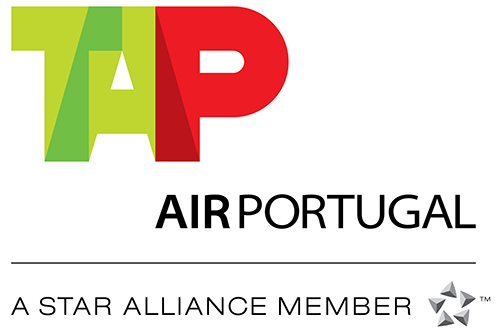
\includegraphics[width=0.5\columnwidth]{logos/tapairpt-logo.png}
\end{center}

\vfill

\section*{Media sponsor}

\begin{center}

\includegraphics[width=0.55\columnwidth]{logos/multilingual-logo.jpg}
\end{center}

\vfill

\section*{Institutional partners}

\begin{center}

\includegraphics[width=0.6\columnwidth]{logos/ist-logo.png}\\


\includegraphics[width=0.6\columnwidth]{logos/inescid-logo.png}
\end{center}

\end{document}
